% !TEX TS-program = XeLaTeX
% use the following command:
% all document files must be coded in UTF-8
\documentclass[spanish]{textolivre}
% build HTML with: make4ht -e build.lua -c textolivre.cfg -x -u article "fn-in,svg,pic-align"

\journalname{Texto Livre}
\thevolume{16}
%\thenumber{1} % old template
\theyear{2023}
\receiveddate{\DTMdisplaydate{2022}{12}{23}{-1}} % YYYY MM DD
\accepteddate{\DTMdisplaydate{2023}{3}{16}{-1}}
\publisheddate{\DTMdisplaydate{2023}{4}{20}{-1}}
\corrauthor{Jorge Oceja}
\articledoi{10.1590/1983-3652.2023.42234}
%\articleid{NNNN} % if the article ID is not the last 5 numbers of its DOI, provide it using \articleid{} commmand 
% list of available sesscions in the journal: articles, dossier, reports, essays, reviews, interviews, editorial
\articlesessionname{articles}
\runningauthor{Oceja y Obregón Sierra} 
%\editorname{Leonardo Araújo} % old template
\sectioneditorname{Hugo Heredia Ponce}
\layouteditorname{Thaís Coutinho}

\title{Los videojuegos independientes en Wikipedia:
análisis de las referencias utilizadas para representar juegos con posibilidades educativas}
\othertitle{Videogames independentes na Wikipedia:
análise das referências utilizadas para representar jogos com possibilidades educativas}
\othertitle{Indie Games in Wikipedia: analysis of the references used to frame games with educational possibilities}
% if there is a third language title, add here:
%\othertitle{Artikelvorlage zur Einreichung beim Texto Livre Journal}

\author[1]{Jorge Oceja~\orcid{0000-0003-2377-9523}\thanks{Email: \href{mailto:jorge.oceja@unican.es}{jorge.oceja@unican.es}}}
\author[2]{Ángel Obregón Sierra~\orcid{0000-0001-8801-317X}\thanks{Email: \href{mailto:angel.obregon@ui1.es}{angel.obregon@ui1.es}}}
\affil[1]{Universidad de Cantabria, Facultad de Educación, Cantabria, España.}
\affil[2]{Universidad Isabel I, Facultad de Educación, Burgos, España.}

\addbibresource{article.bib}
% use biber instead of bibtex
% $ biber article

% used to create dummy text for the template file
\definecolor{dark-gray}{gray}{0.35} % color used to display dummy texts
\usepackage{lipsum}
\SetLipsumParListSurrounders{\colorlet{oldcolor}{.}\color{dark-gray}}{\color{oldcolor}}

% used here only to provide the XeLaTeX and BibTeX logos
\usepackage{hologo}

% if you use multirows in a table, include the multirow package
\usepackage{multirow}

% provides sidewaysfigure environment
\usepackage{rotating}

% CUSTOM EPIGRAPH - BEGIN 
%%% https://tex.stackexchange.com/questions/193178/specific-epigraph-style
\usepackage{epigraph}
\renewcommand\textflush{flushright}
\makeatletter
\newlength\epitextskip
\pretocmd{\@epitext}{\em}{}{}
\apptocmd{\@epitext}{\em}{}{}
\patchcmd{\epigraph}{\@epitext{#1}\\}{\@epitext{#1}\\[\epitextskip]}{}{}
\makeatother
\setlength\epigraphrule{0pt}
\setlength\epitextskip{0.5ex}
\setlength\epigraphwidth{.7\textwidth}
% CUSTOM EPIGRAPH - END

% LANGUAGE - BEGIN
% ARABIC
% for languages that use special fonts, you must provide the typeface that will be used
% \setotherlanguage{arabic}
% \newfontfamily\arabicfont[Script=Arabic]{Amiri}
% \newfontfamily\arabicfontsf[Script=Arabic]{Amiri}
% \newfontfamily\arabicfonttt[Script=Arabic]{Amiri}
%
% in the article, to add arabic text use: \textlang{arabic}{ ... }
%
% RUSSIAN
% for russian text we also need to define fonts with support for Cyrillic script
% \usepackage{fontspec}
% \setotherlanguage{russian}
% \newfontfamily\cyrillicfont{Times New Roman}
% \newfontfamily\cyrillicfontsf{Times New Roman}[Script=Cyrillic]
% \newfontfamily\cyrillicfonttt{Times New Roman}[Script=Cyrillic]
%
% in the text use \begin{russian} ... \end{russian}
% LANGUAGE - END

% EMOJIS - BEGIN
% to use emoticons in your manuscript
% https://stackoverflow.com/questions/190145/how-to-insert-emoticons-in-latex/57076064
% using font Symbola, which has full support
% the font may be downloaded at:
% https://dn-works.com/ufas/
% add to preamble:
% \newfontfamily\Symbola{Symbola}
% in the text use:
% {\Symbola }
% EMOJIS - END

% LABEL REFERENCE TO DESCRIPTIVE LIST - BEGIN
% reference itens in a descriptive list using their labels instead of numbers
% insert the code below in the preambule:
%\makeatletter
%\let\orgdescriptionlabel\descriptionlabel
%\renewcommand*{\descriptionlabel}[1]{%
%  \let\orglabel\label
%  \let\label\@gobble
%  \phantomsection
%  \edef\@currentlabel{#1\unskip}%
%  \let\label\orglabel
%  \orgdescriptionlabel{#1}%
%}
%\makeatother
%
% in your document, use as illustraded here:
%\begin{description}
%  \item[first\label{itm1}] this is only an example;
%  % ...  add more items
%\end{description}
% LABEL REFERENCE TO DESCRIPTIVE LIST - END


% add line numbers for submission
%\usepackage{lineno}
%\linenumbers

\begin{document}
\maketitle

\begin{polyabstract}
\begin{abstract}
La diversidad en la industria de los videojuegos se manifiesta en una escena independiente que ha generado obras artísticas con grandes posibilidades educativas. El presente trabajo parte de una selección de 36 juegos independientes y analiza el contenido de sus artículos en Wikipedia. Se centra en las referencias que contienen dichos artículos para entender cómo son representados los juegos en este medio. Tras comprobar que 28 de estos juegos poseen artículos en Wikipedia, se obtuvieron las referencias bibliográficas ($n = 2058$) identificado cada uno de los medios con los que se nutren estos artículos y clasificándolos en función de sus características. Los resultados muestran que los artículos varían en extensión, siendo \emph{Life is Strange} el más amplio (120621 bytes) y el que contiene más referencias (185). Se observó también que el 61,5\% de estas referencias corresponden a revistas y páginas sobre videojuegos y el 20,9\% a otras de carácter más generalista. Los datos confirman que la mayoría de los artículos están construidos con fuentes de escaso rigor académico, lo que dificulta la exploración de las posibilidades educativas de estos juegos. Llama la atención la ausencia de libros, actas de congresos o revistas científicas, en particular del ámbito educativo, los \textit{games studies} o el aprendizaje basado en juegos.

\keywords{Juegos independientes \sep Indie games \sep Aprendizaje basado en juegos \sep Wikipedia}
\end{abstract}

\begin{portuguese}
\begin{abstract}
A diversidade na indústria de videogames se manifesta em uma cena independente que tem gerado obras artísticas com grandes possibilidades educativas. Este artigo se baseia em uma seleção de 36 jogos independentes e analisa o conteúdo de seus artigos na Wikipédia. Centra-se nas referências contidas nesses artigos para entender como esses jogos são representados nesse meio. Depois de verificar que 28 desses jogos possuem artigos na Wikipedia, foram obtidas as referências bibliográficas ($n = 2058$), identificando cada uma das mídias com as quais esses artigos são alimentados e classificando-os de acordo com suas características. Os resultados mostram que os artigos variam em extensão, sendo \textit{Life is Strange} o maior (120621 bytes) e o que contém mais referências (185). Observou-se ainda que 61,5\% dessas referências correspondem a revistas e páginas sobre videojogos e 20,9\% a outras de carácter mais geral. Os dados confirmam que a maioria dos artigos é construída com fontes de pouco rigor acadêmico, o que dificulta a exploração das possibilidades educacionais desses jogos. Chama a atenção a ausência de livros, anais de conferências ou revistas científicas, principalmente no campo educacional, \textit{game studies} ou aprendizagem baseada em jogos.

\keywords{Videogames independentes \sep Indie games \sep Aprendizagem baseada em jogos \sep Wikipédia}
\end{abstract}
\end{portuguese}

\begin{english}
\begin{abstract}
Diversity in the video game industry has led to a vibrant independent scene full of artistic products with great educational possibilities. This work analyzes 36 independent games and their Wikipedia articles focusing on their bibliographic references to understand how are they framed. After confirming that 28 of these games have Wikipedia articles, references were obtained ($n = 2058$) and each individual media was identified and classified based on their characteristics. Results show that articles differ in legth, with \emph{Life is Strange} being the largest (120621 bytes) and the one with more references (185 references). 61,5\% of the total references come from magazines and websites focusing on games, while 20,9\% correspond to more general media. Data shows that most articles contain sources of dubious quality, which complicates the exploration of the educational possibilities of these games. It is remarkable the absence of books, conference proceedings and academic journals, especially those from the educational field, game studies or game-based learning.
 
\keywords{Independent video games \sep Indie games \sep Game based learning \sep Wikipedia}
\end{abstract}
\end{english}
% if there is another abstract, insert it here using the same scheme
\end{polyabstract}

\section{Introducción}
\subsection{Videojuegos y educación. Una larga historia sin resolver}
Los videojuegos son un medio convergente o medio de medios que combina elementos narrativos propios de otros lenguajes (como el cine o la literatura) con una dimensión lúdica que surge, muchas veces, de la interacción que el sistema ofrece al jugador. Aunque han sido utilizados en educación desde su aparición en la década de los años 70 \cite{jones2017}, es interesante repasar cuáles han sido estos usos y qué tipo de juegos ha promovido cada enfoque. En este sentido, posiblemente la variable más importante ha sido la teoría de aprendizaje predominante en cada época. Por ejemplo, tal y como apuntan algunos autores \cite{facer2003}, en los años 60 los acercamientos conductistas gozaban de un gran crédito y la interpretación del individuo como un emisor de respuestas ante determinados estímulos parecía encajar con el nuevo medio. Aparecieron esos años multitud de juegos (muchas veces vinculados al área de matemáticas) basados en preguntas o tareas simples que ofrecían al jugador recompensas cada vez que completaba una operación de forma satisfactoria. En juegos como \emph{Mathblaster}, se ofrecía incluso como recompensa la posibilidad de seguir jugando, convirtiéndose la actividad en el propio premio extrínseco para promocionar un comportamiento. Aunque algunos autores se han referido a estos acercamientos como eduentretenimiento \cite{egenfeldt2021understanding}, tradicionalmente han gozado de una gran popularidad y siguen teniendo protagonismo en el ámbito del aprendizaje basado en juegos. En particular, el reciente auge de la gamificación ha revitalizado estos acercamientos fascinando, sin explicación aparente, a instituciones y profesionales de la educación \cite{oceja_business_2022}.

La posterior consolidación de los enfoques cognitivistas \cite{egenfeldt2021understanding} destapó esa caja negra para prestar atención a los procesos internos de los sujetos, atendiendo a variables como la atención, la motivación o la memoria. Esto coincidió con cierto reconocimiento de los videojuegos como productos culturales complejos. Si bien las posibilidades del medio seguían sin ser explotadas, al menos comenzaba a reconocerse su potencial educativo, más allá de ser un expendedor de recompensas.

Los acercamientos constructivistas, por su parte, siempre se han explicado a partir de la metáfora del andamiaje \cite{piaget_psicologinino_1997}. El foco dejó de ponerse en el procesamiento mecanicista de la información, centrándose en la interacción de los sujetos con el medio y en la reconstrucción de sus esquemas cognitivos a través de la asimilación (la integración de lo nuevo en esos esquemas) y la acomodación (la modificación de los esquemas previos para integrar de forma coherente la nueva información) \cite{piaget_psicologinino_1997}. Esto, en el ámbito de los juegos, se traduciría en mundos abiertos en los cuales el jugador pueda interaccionar de forma libre con el entorno. Aunque el éxito educativo de juegos como \emph{Minecraft} \cite{nebel2016mining} sería representativo de esta línea, muchas veces estas prácticas han servido para trabajar contenidos aritméticos o espaciales de una forma convencional. Por su parte, el construccionismo, una subteoría del constructivismo \cite{papert_mindstorms:_1983} iría más allá al afirmar que la interacción productiva no ocurre cuando los alumnos juegan sino cuando se involucran en los procesos de diseño. El éxito de proyectos como \emph{The Hour of The Code} \cite{yauney_systematic_2022} o la utilización de Scratch en las escuelas \cite{fagerlund_computational_2021} serían representativos de este tipo de acercamientos.

Finalmente, es necesario referirse a los acercamientos socioculturales, abanderados por \textcite{gee_what_214}. Según estos enfoques la intencionalidad educativa no es el elemento más importante de la experiencia, sino el contexto en el que los juegos son jugados y las conversaciones a las que da lugar el acto de jugar. Estos acercamientos dialógicos reivindican la utilización de juegos comerciales \cite{lave_situated_1991} sin un sentido educativo \emph{per} se. Aunque pueden existir juegos explicitamente educativos bien diseñados \cite{del2012evaluacion}, los enfoques socioculturales subrayarían, en la línea apuntada por algunos autores \cite{lopez2016experiencias}, las posibilidades que ofrecen los juegos comerciales. Entenderían, por lo tanto, los juegos como productos que, al igual que el cine, el cómic o la literatura son susceptibles de ser llevados a las aulas por el hecho de ser manifestaciones artísticas y culturales.

Esta asociación entre las teorías clásicas de aprendizaje y los usos educativos de los juegos guarda relación con el esquema generado por \textcite{plass_foundations_2015} en lo que denominan \emph{Marco para el diseño integrado de aprendizajes lúdicos}. Si bien su trabajo pretende ser una guía de diseño de experiencias educativas lúdicas, menciona cuatro tipos de \emph{engagement} que pueden ocurrir cuando se aprende a través de juegos: afectivo, comportamental, cognitivo y sociocultural. Tres de ellos se corresponderían con lo que proponen, a grandes rasgos, las teorías mencionadas (conductismo, cognitivismo y acercamientos socioculturales) añadiendo, además, una dimensión clave como es la emocional. En este trabajo reivindicamos las posibilidades que ofrecen los juegos para trabajar el ámbito afectivo-emocional, y por ello consideramos esta cuestión particularmente interesante.

De todos los géneros y productos en los que se manifiesta la diversidad y creatividad del medio, el ámbito independiente es el que ofrece obras con un mayor carácter artístico \cite{perez_latorre_indie_2016} y, por extensión, mayores posibilidades para el trabajo afectivo-emocional y curricular en el aula.


\subsection{Los juegos independientes y el aprendizaje afectivo-emocional desde perspectivas socioculturales}
El hecho de que los juegos independientes sean desarrollados por pequeños equipos (en ocasiones por un solo diseñador) ha llevado a algunos autores a referirse a ellos como juegos de autor \cite{backe_within_2017}. Al igual que ocurre con el cine, la música o la literatura independiente, la autonomía y libertad de los autores da lugar a artefactos únicos, con un marcado carácter poético, ideales para la generación de aprendizajes dialógicos.

Se ha debatido si el término independiente está más vinculado a la financiación de los proyectos o a los niveles de libertad creativa de los diseñadores \cite{perez_latorre_indie_2016}. En nuestra opinión ambas cuestiones van de la mano, llevando a los autores a implicarse en la creación de obras personales que exploran las posibilidades expresivas del medio. Aunque estos juegos quedan muchas veces al margen de los canales comerciales, en los últimos años hemos presenciado excepciones notorias como \emph{Minecraft}, desarrollado por Markus Persson, Journey de la compañía Thatgamecompany o, en el contexto hispano, \emph{Gris} de Nómada Studio o \emph{RiME} de Tequila Works. Las características mencionadas hacen que estos juegos sean particularmente útiles para trabajar, además de contenidos curriculares, la dimensión afectivo-emocional, cuya importancia ha sido subrayada desde distintos modelos teóricos \cite{bar2006bar, mayer_ability_2016}. Además, tal y como indican \textcite{plass_foundations_2015}, los resultados más prometedores en esta línea ocurren cuando trabajamos bajo enfoques socioculturales y dialógicos. Sin embargo, apenas existen trabajos que hayan utilizado estos acercamientos para llevar al aula los juegos independientes.


\subsection{Representación de los juegos independientes en Wikipedia}
Desde sus orígenes, tanto Wikipedia como Wikidata han mostrado una gran capacidad para recoger información sobre videojuegos. Por ejemplo, una búsqueda en Wikidata Query Service, el servicio de consultas de Wikidata, con la cadena que aparece en la \Cref{fig01} (\url{https://w.wiki/5xFc}) muestra que, en noviembre de 2022 había 54248 juegos introducidos en la base de datos, de los cuales 26506 tenían asociado al menos un artículo en la versión en inglés de Wikipedia. Lo interesante de Wikidata no es tanto la cantidad de juegos almacenados, sino el entramado de personajes, creadores, estudios y empresas asociadas a esos juegos y que también aparecen documentados.

\begin{figure}[htbp]
\centering
\begin{minipage}{.85\textwidth}
 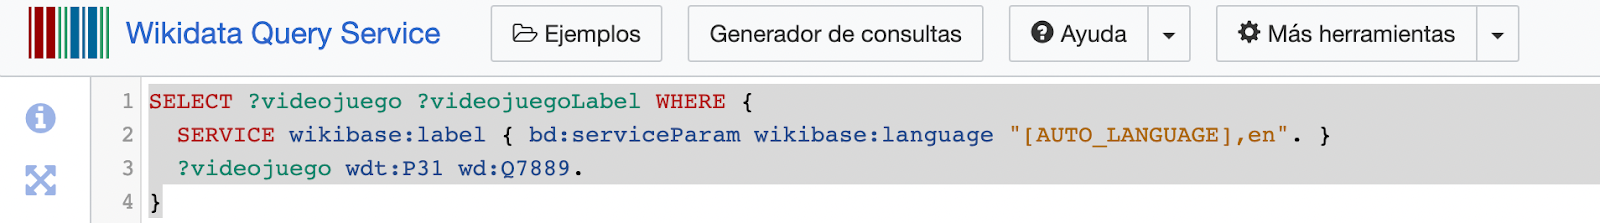
\includegraphics[width=\textwidth]{Fig01.png}
 \caption{Búsqueda realizada en Wikidata Query Service para obtener el número de juegos introducidos en Wikidata}
 \label{fig01}
 \source{Wikidata}
\end{minipage}
\end{figure}

Cada artículo de Wikipedia se basa en citas y referencias que aparecen colocadas al final de cada página, como ocurre con los trabajos de corte académico. Por lo tanto, Wikipedia no es una fuente de información primaria ya que su contenido debe nutrirse de otras fuentes para así mejorar su fiabilidad \cite{wikiciting7}. Aunque la mayoría de estudios sobre la calidad de los contenidos se da en temas relacionados con la medicina (dado al riesgo de que los lectores accedan a fuentes de baja calidad), existen algunos centrados en otras temáticas. Por ejemplo, se ha estudiado la calidad de los contenidos en temas tan dispares como las universidades \cite{claes_wikipedia_2020}, el periodismo \cite{morejon_llamas_mujeres_2021}, la estadística \cite{dunn_evaluating_2019} y la nutrición \cite{carrera_presence_2015}. Sin embargo, no existe información acerca de la calidad de los artículos sobre videojuegos en Wikipedia y, menos aún, sobre juegos independientes que, por sus características y por lo explicado en el marco de este trabajo, pudieran ofrecer posibilidades en el ámbito educativo.

Por todo ello, el problema que guía este trabajo es la ausencia de datos sobre cómo estos juegos son representados en Wikipedia y cuál es la naturaleza de los medios en los que se basan esos artículos.

Para atender este problema se intenta dar respuesta a cuatro preguntas de investigación. En primer lugar, (1) cuál es la presencia de los juegos independientes en Wikipedia y cómo se ordenarían sus artículos de acuerdo a dos variables (cantidad de información generada y número de referencias de cada artículo). En segundo lugar, (2) en qué medida existe una correlación entre el tamaño de los artículos y la cantidad de referencias que contienen, analizando también si la fecha de creación afecta a su extensión. En tercer lugar, (3) cuáles son los principales medios utilizados por los editores como referencias para crear estos artículos. Finalmente, (4) cuál es la naturaleza de estos medios para confirmar o descartar si se utilizan fuentes de calidad en la construcción de dichos artículos.



\section{Metodología}
Para seleccionar la muestra de videojuegos y sus correspondientes artículos, recurrimos a dos de los principales eventos en el ámbito de los juegos independientes y/o juegos con posibilidades educativas: el \emph{Independent Game Festival} (\url{https://igf.com}) y la iniciativa \emph{Games for Change} (\url{https://www.gamesforchange.org}). Esto nos permitió combinar juegos independientes con posibilidades educativas explícitas (\emph{Games for Change}) con juegos de carácter artístico que, si bien pueden haber sido diseñados sin una intencionalidad educativa, dadas sus peculiaridades y el posicionamiento de este trabajo, podrían utilizarse en contextos educativos. Esto también nos permitió explorar si la selección de juegos coincidía y, por extensión, eliminar posibles redundancias.

\emph{Games for Change} es una organización sin ánimo de lucro fundada en 2014 en Nueva York con la intención de apoyar a los diseñadores de juegos y a emprendedores para que generen un impacto social a través de los juegos y los medios inmersivos. Cada año seleccionan juegos en función de categorías como juego del año (GOTY), impacto más significativo (MSI), mejor jugabilidad (BG) o juego más innovador (MI). Decidimos incluir la mayoría de juegos galardonados en las distintas categorías con excepciones puntuales como \emph{Nintendo Labo}, al no ser un juego \emph{per} se ni un producto de corte independiente. Tampoco se incluyen productos de corte exclusivamente educativo y/o académico que no puedan ser adquiridos de una forma convencional por los docentes, lo que dejó fuera a juegos como \emph{Unicef Kid Power}. Cuando alguno de los eventos ha propuesto alguna categoría novedosa, si el juego galardonado se enmarcaba en lo expuesto en el trabajo, ha sido incluido en la lista. \emph{Hellblade: Senua’s sacrifice}, vencedor de la categoría GPCA o \emph{Homestay} ganador del premio BXFC son algunos ejemplos.

Para evitar un sesgo que llevara a nuestra selección hacia lo estrictamente educativo o político, añadimos la lista de ganadores del premio al mejor juego del \emph{Independent Games Festival}. Este evento, que tiene lugar durante la \emph{Game Developers Conference}, es considerado uno de los encuentros más importantes del mundo para los desarrolladores de videojuegos independientes. En sus propias palabras “El sentido de este evento es crear algo similar al Festival de Cine de Sundance para diseñadores independientes de videojuegos”.

La \Cref{tab01} presenta los juegos seleccionados en el trabajo mostrando en columnas el evento al que pertenecen.


\begin{table}[h!]
\centering
\begin{threeparttable}
\caption{Juegos premiados en el Games for Change y en el Independent Game Festival desde 2014.}
\label{tab01}
\begin{tabular}{ll}
\toprule
Games for change &
Independent Game Festival \\ 
\midrule

Gone Home (GOTY) & \multirow{3}{*}{Papers, Please} \\
Papers, Please (MI and BG) & \\
Mission us: a cheyenne odyssey (MSI) & \\
\midrule

Never Alone (GOTY and MSI) & \multirow{3}{*}{Outer Wilds}\\ 
This war of mine (BG) & \\ 
Bounden	(MI) & \\
\midrule

Life is Strange (GOTY, MSI)	& \multirow{3}{*}{Her Story}\\ 
Block’hood (BG) & \\ 
That Dragon, Cancer (MI) & \\
\midrule

Walden, A game (GOTY, MSI) & \multirow{3}{*}{Quadrilateral Cowboy}\\
Tracking IDA (BG) & \\ 
Everything (MI) & \\
\midrule

Life is Strange: Before the Storm (GOTY, MSI) & \multirow{4}{*}{Night in the Woods}\\
Tree (MI) & \\
What remains of Edith Finch (BG) & \\ 
Hellblade: Senua’s sacrifice (GPCA) & \\
\midrule

Gris (BG) & \multirow{3}{*}{Return of the Obra Dinn}\\
Tendar (MI) & \\ 
Homestay (BXFCE) & \\
\midrule

Dreams (GOTY and MI) & \multirow{3}{*}{A Short Hike}\\ 
Sea of solitude (MSI) & \\ 
Sky: Children of the light (BG) & \\
\midrule

Lost Words: Beyond the Page (MI y BG) & \multirow{2}{*}{Umurangi Generation}\\ 
Alba: A wildlife adventure (GOTY and MSI) & \\
\midrule

Dot’s Home (GOTY) & \multirow{4}{*}{Inscryption}\\
The Vale: Shadow of the Crown (MI) & \\
Svoboda 1945: Liberation (MSI) & \\ 
Before your eyes (BG) & \\
\bottomrule
\end{tabular}
\source{Elaboración propia}
\end{threeparttable}
\end{table}

Como puede observarse, \emph{Papers, Please} es el único videojuego que aparece en los dos premios. Tras la eliminación de datos redundantes trabajamos con 36 juegos.


\subsection{Bytes generados y cantidad de referencias}
En primer lugar, se obtuvo el número de bytes de cada artículo a partir de la información que aparece en los históricos de Wikipedia. Se procedió de forma manual para identificar los valores en cada uno de ellos.

La forma en la que Wikipedia maneja las referencias de sus artículos es más complicada, al ofrecer a los editores distintas plantillas con diversos campos a la hora de crear los artículos. Entre estas nos encontramos Cite book, Cite magazine, Cite news, Cite web e incluso una dedicada a los videojuegos (Cite videogame) \cite{wikiciting7}. Por su parte, otros editores prefieren añadir las fuentes sin utilizar plantillas, insertando todos los parámetros de forma manual \cite{wikicitinginline}.

Este proceso puede simplificarse usando un editor visual o incluso copiando el código de las páginas de ayuda para adaptarlo después. En el presente trabajo, para recoger la información de las referencias de cada artículo, desarrollamos y ejecutamos un script programado en PHP. El script accedió a los artículos de Wikipedia recogiendo todas las apariciones de la etiqueta “<ref>”, guardando en ese caso el nombre del juego y el contenido de cada referencia.

\subsection{Estrategias para el análisis de datos}
Para clasificar las referencias de los artículos fue necesario adoptar una taxonomía de medios. Esta cuestión siempre ha resultado compleja en ciencias de la comunicación dados los diferentes criterios que pueden aplicarse: formato del medio, materia, canal, etc. Posiblemente, el intento clasificatorio más conocido es el de \textcite{beth1990introduccion} al diferenciar entre medios primarios, vinculados al cuerpo humano (teatro, comunicación oral, etc.), medios secundarios, vinculados a lo electrónico (periódicos, revistas, etc.) y medios terciarios, vinculados lo electrónico (televisión, radio, etc.). Más tarde, \textcite{rehberg_informationelle_1997} añadiría una cuarta categoría que denominó medios cuaternarios y que estaría asociada a lo digital incluyendo, sobre todo, Internet.

Aunque valoramos estos intentos clasificatorios, ambos presentan problemas, dado que cruzan criterios vinculados al formato (físico vs. digital) con otros asociados al tipo de producto (periódico, revista, etc.). Dados estos solapamientos, también consideramos usar el sistema clasificatorio de la propia Wikipedia. En él, las categorías aparecen ordenadas de forma jerárquica, sirviendo para agrupar, organizar y permitir la búsqueda de artículos \cite{gangemi_tagtheweb:_2018}.

\begin{figure}[htbp]
\centering
\begin{minipage}{.85\textwidth}
 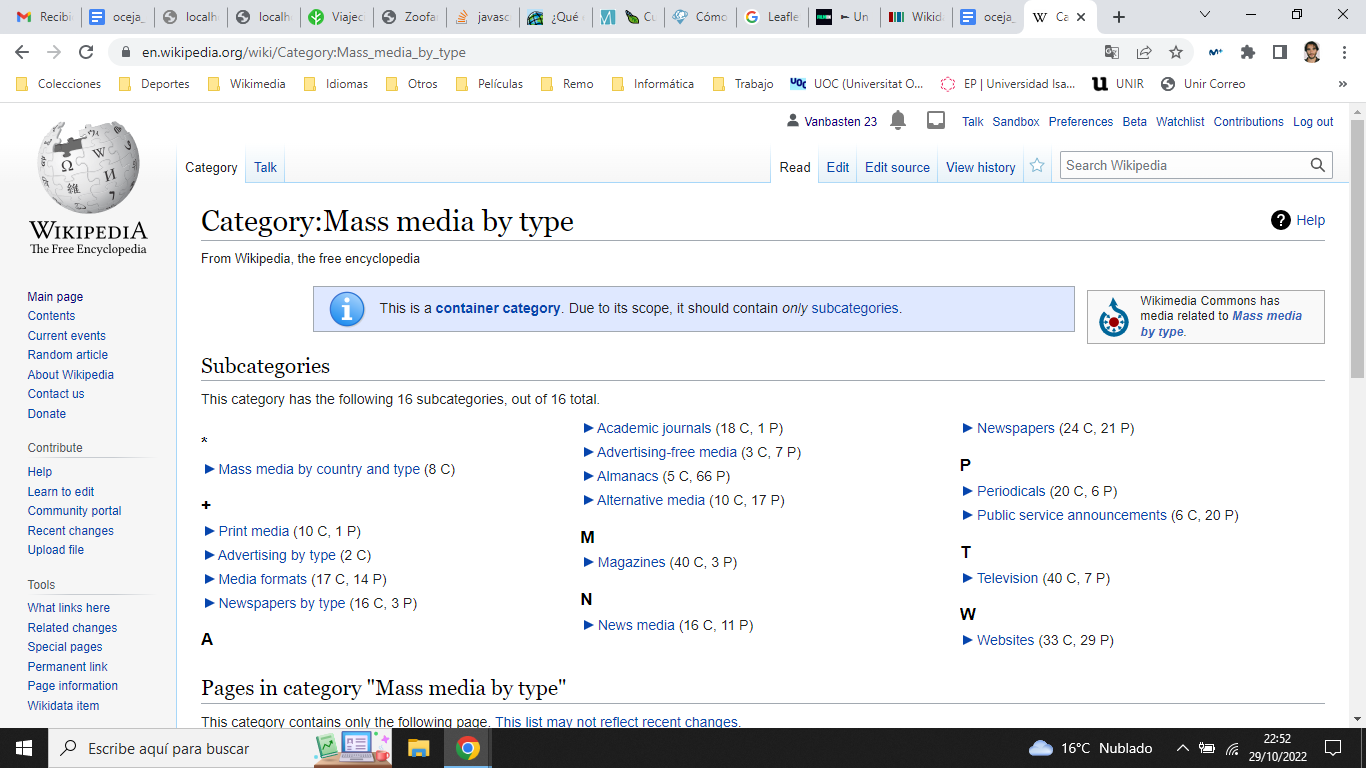
\includegraphics[width=\textwidth]{fig02.png}
 \caption{Categoría Mass media by type en Wikipedia en inglés}
 \label{fig02}
 \source{Wikipedia}
\end{minipage}
\end{figure}

Como puede verse en la \Cref{fig02}, comenzando con la categoría “Mass media by type” encontramos subcategorías que parecerían pertinentes para nuestro trabajo, como “Televisión”, “Periódicos”, “Revistas”, “Revistas académicas”, etc. Sin embargo, también aparecen otras como “Páginas web de noticias” (que a su vez contiene otra subcategoría denominada “Páginas web de noticias sobre videojuegos”), “Noticias de televisión”, “Noticias de radio”, “Noticias de podcast”, “Periódicos” y “Noticias de revistas”.

Aunque la propuesta vuelve a ser interesante, aparecen solapamientos y distinciones que a día de hoy no son aplicables. Un ejemplo es la distinción entre “Noticias de revistas” y “Noticias de páginas web” en un contexto en el que muchos medios generan versiones tanto en papel como en digital.

Además, es importante destacar que en el propio proceso de recogida de datos emergieron de forma inductiva categorías novedosas. Algunos ejemplos son aplicaciones de foros, páginas de eventos y premios o las propias páginas web de los juegos seleccionados.

Combinando estos acercamientos e intentando superar sus limitaciones (siendo conscientes de que cualquier intento es imperfecto por naturaleza) el sistema clasificatorio con el que trabajamos fue el siguiente:

\begin{itemize}
  \item Medios de noticias:
  \begin{itemize}
    \item Revistas y páginas web.
    \begin{itemize}
      \item Sobre noticias generalistas o no centradas en videojuegos.
      \item Sobre noticias específicas de videojuegos.
    \end{itemize}
    \item Televisión.
    \item Periódicos.
    \item Radio.
  \end{itemize}
\end{itemize}

\begin{itemize}
  \item Medios académicos.
  \begin{itemize}
    \item Libros académicos.
    \item Revistas académicas.
  \end{itemize}
\end{itemize}

\begin{itemize}
    \item Foros.
    \item Páginas oficiales de juegos y/o diseñadores.
    \item Otras fuentes emergentes:
    \begin{itemize}
        \item Premios y festivales.
        \item Charlas y conferencias.
        \item Páginas de los fabricantes de equipos (consolas, ordenadores etc.).
    \end{itemize}
\end{itemize}






\subsection{Estrategias para el análisis de datos}
Para dar respuesta a la primera pregunta de investigación se recogieron los bytes y el número de referencias de cada artículo para determinar cuantitativamente el tamaño de cada uno y la cantidad de medios de los que se nutre. Posteriormente se generó un gráfico de barras ordenando cada artículo de mayor a menor incluyendo ambos valores.

En lo relativo a la segunda pregunta de investigación, se utilizó el software de análisis estadístico R con el objetivo de comprobar si existía una correlación directa entre el tamaño de cada artículo y el número de referencias que contiene. De esta forma comprobaríamos la hipótesis, a priori lógica, de que cuantas más referencias, más grande será el artículo.

Con intención de dar respuesta a la tercera pregunta de investigación se generó una tabla con un listado de los diez medios más utilizados como referencias por los editores, incluyendo además el número de veces que aparecía cada uno.

Finalmente, para la cuarta pregunta de investigación se utilizó el sistema clasificatorio propuesto. En primer lugar, se generó un documento abierto con la extensión .csv que contenía todas las referencias de los artículos indicando a qué categoría correspondía cada medio. En función del peso final de cada categoría de medios (determinado en función del número de referencias que se ubicaban en esa categoría) se creó un gráfico circular para representar la importancia de cada categoría, sintetizando qué tipo de medios usan los editores para construir sus artículos.


\section{Resultados}

En primer lugar, se comprobó cuántos de los 36 juegos estaban dentro de los proyectos de la Fundación Wikimedia. Para ello se realizó una búsqueda en Wikidata, encontrando elementos para 30 de ellos. Se constató que Wikipedia en inglés era la versión idiomática que representaba estos juegos de forma más exhaustiva, al dedicar artículos a 28 de ellos, tal y como puede observarse en la \Cref{tab02}:

\begin{table}[h!]
\centering
\begin{threeparttable}
\caption{Presencia de los juegos premiados en los proyectos de la Fundación Wikimedia}
\label{tab02}
\begin{tabular}{lll}
\toprule
Juego                            & Wikidata   & Idiomas \\ 
\midrule
Life 			is Strange               & Q18536861  & 34      \\ 
Hellblade: Senua’s...             & Q18185763  & 19      \\ 
Life 			is Strange: Before...     & Q30242632  & 24      \\ 
Her 			Story                     & Q20538669  & 13      \\ 
Night 			in the Woods            & Q19383244  & 16      \\ 
Dreams                           & Q22000976  & 13      \\ 
Gone 			Home                     & Q5581572   & 12      \\ 
Papers, 			Please                & Q14565978  & 30      \\ 
Outer 			Wilds                   & Q19631660  & 12      \\ 
What 			remains of Edith...      & Q28451186  & 15      \\ 
Sky: Children 			of the light     & Q64547527  & 16      \\ 
This 			war of mine              & Q16743212  & 21      \\ 
That 			Dragon, Cancer           & Q16267891  & 6       \\ 
Return 			of the Obra Dinn       & Q48987695  & 13      \\ 
Gris                             & Q59769284  & 12      \\ 
Everything                       & Q29057412  & 5       \\ 
Never 			Alone                   & Q17512815  & 9       \\ 
Inscryption                      & Q109051201 & 6       \\ 
Walden, 			A game                & Q46993159  & 1       \\ 
Quadrilateral 			Cowboy          & Q7268403   & 2       \\ 
A 			Short Hike                  & Q66035140  & 8       \\ 
Before 			your eyes              & Q106452472 & 1       \\ 
Sea 			of solitude               & Q28196135  & 6       \\ 
Umurangi 			Generation           & Q104634041 & 2       \\ 
Block’hood                       & Q23024065  & 1       \\ 
Alba: 			A wildlife adventure    & Q104529092 & 1       \\ 
Lost 			Words: Beyond...         & Q90008611  & 1       \\ 
Bounden                          & Q18643685  & 3       \\ 
Svoboda 			1945: Liberation      & Q111443969 & 1       \\ 
The 			Vale: Shadow of the Crown & Q108169836 & 0       \\ 
\bottomrule
\end{tabular}
\source{Elaboración propia (2022)}
\end{threeparttable}
\end{table}

Tras la versión en inglés, aparecen el resto de idiomas: francés (22), ruso (17), italiano (16), chino (15), árabe (15), persa (14), portugués (14), japonés (13), alemán (13) y español (12). Los únicos artículos que no existen en la versión en inglés son \emph{Mission us: a Cheyenne odyssey, Tracking IDA, Tree, Tendar, Homestay, Dot’s Home, The Vale: Shadow of the Crown y Svoboda 1945: Liberation}, aunque estos dos últimos sí tienen elemento en Wikidata.

La \Cref{fig03} recoge los artículos sobre los juegos seleccionados en este estudio, ordenados en función del número de bytes y el número de referencias utilizadas.

\begin{figure}[htbp]
\centering
\begin{minipage}{.85\textwidth}
 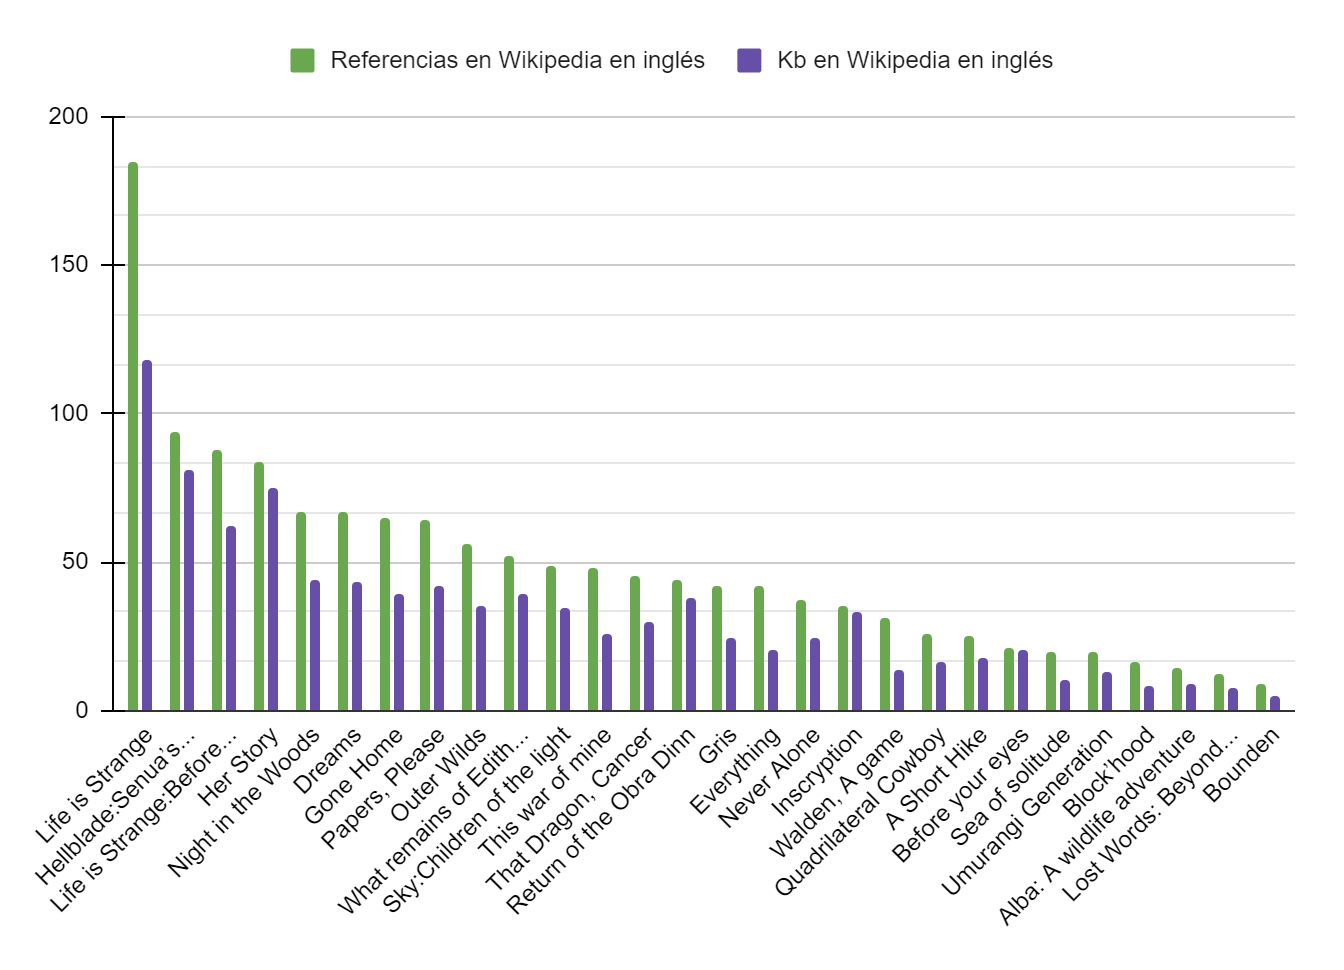
\includegraphics[width=\textwidth]{fig03.png}
 \caption{Listado de los 28 juegos seleccionados, ordenados en función de su tamaño y del número de referencias que incluye}
 \label{fig03}
 \source{Elaboración propia}
\end{minipage}
\end{figure}

Si atendemos al número de bytes y al número de referencias, el juego más importante es \emph{Life is Strange} (120621 bytes y 185 referencias). Este artículo ha sido editado por 580 usuarios, se ha visto 9386 veces (447 de promedio diario) y se ha editado en un total de 2582 ocasiones. Por detrás encontramos a \emph{Hellblade: Senua's Sacrifice} (83203 bytes y 94 referencias) y \emph{Her Story} (76804 bytes y 84 referencias), el primer juego indie en un sentido estricto si atendemos al tamaño de los equipos de desarrollo. \emph{Hellblade} ha sido editado por 263 usuarios diferentes, que han realizado 651 ediciones, mientras \emph{Her Story} ha sido editado por 120 editores en 297 ocasiones.

El caso de \emph{Life is Strange} es interesante porque una de sus continuaciones (\emph{Life is Strange: Before the Storm}) cuarta en número de bytes y tercera en referencias (63506 bytes y 88 referencias).

El resto de juegos analizados se mueven entre 12 y 67 referencias y entre 7876 y 45106 bytes, hasta llegar al último de la lista (\textit{Bounden}), el juego desarrollado por la Compañía Nacional de Danza de Países Bajos (5035 bytes y 9 referencias). 

Para dar respuesta a la segunda pregunta de investigación, comprobamos la correlación existente entre el número de referencias y el número de bytes de cada artículo. Aunque parecía evidente que a mayor tamaño de los artículos mayor número de referencias, este extremo debía ser confirmado. Para ello calculamos los coeficientes de Pearson ($r = 0.8587$, $p < 001$) y Spearman ($r = 0.9691$, $p < 001$) constatando que según los criterios de Rumsey (2015) esta era elevada.

Para ver la relación entre las dos variables también se creó el diagrama de dispersión con su línea de tendencia en R, mostrando en el eje X las referencias y en el eje Y los bytes (\Cref{fig04}).

\begin{figure}[htbp]
\centering
\begin{minipage}{.85\textwidth}
 
\includegraphics[width=\textwidth]{fig04.png}
 \caption{Diagrama de dispersión con su línea de tendencia entre las referencias y los bytes de los artículos seleccionados}
 \label{fig04}
 \source{Elaboración propia}
\end{minipage}
\end{figure}

Puede apreciarse que los artículos se encuentran muy cerca de la línea de tendencia en el diagrama de dispersión. Esto nos indica que aquellos que son más grandes tienen más referencias y viceversa, lo que apuntaría a que los primeros están mejor documentados o, al menos, contienen un mayor número de citas. También es necesario entender que las propias referencias ocupan espacio y aumentan los bytes del artículo en el que se encuentran.

Dado que los editores han tenido menos tiempo para trabajar en los juegos más recientes, quisimos analizar si la fecha de publicación tenía alguna influencia en el tamaño del artículo y en la cantidad de referencias. Para ello se obtuvieron los valores de la correlación entre la fecha y las referencias (Pearson: $r = -0.3430$, $p < 001$ y Spearman: $r = -0.3526$, $p < 001$) y entre esta y los bytes (Pearson: $r = -0.2129$, $p < 001$ y Spearman: $r = -0.2339$, $p < 001$). Según Rumsey (2015) esta correlación sería débil, por lo que artículos más recientes no implicarían siempre trabajos más pequeños.

A continuación, se analizaron las referencias que aparecían en los artículos. Los 28 artículos de Wikipedia en inglés presentaban un total de 2058 referencias, aunque 700 correspondían a citas redundantes, por lo que finalmente trabajamos con 1358. La media de referencias aportadas por artículo se sitúa en 73,5.

La \Cref{tab03} muestra los 10 medios que aparecen utilizados más frecuentemente como referencias.

\begin{table}[h!]
\centering
\begin{threeparttable}
\caption{Los 10 medios más usados en la construcción de artículos sobre juegos independientes}
\label{tab03}
\begin{tabular}{llp{7cm}l}
\toprule
Posición & Medio & Categoría & Número de veces \\ 
\midrule
1 & Metacritic & Medios de noticias / Revistas y páginas web / Sobre noticias generalistas & 97 \\ 
2 & Polygon & Medios de noticias / Revistas y páginas web / Sobre noticias específicas de videojuegos & 90 \\
3 & Gamespot & Medios de noticias / Revistas y páginas web / Sobre noticias específicas de videojuegos & 76 \\
4 & Ign & Medios de noticias / Revistas y páginas web / Sobre noticias específicas de videojuegos & 66 \\ 
5 & Eurogamer & Medios de noticias / Revistas y páginas web / Sobre noticias específicas de videojuegos & 61 \\ 
6 & Pcgamer & Medios de noticias / Revistas y páginas web / Sobre noticias específicas de videojuegos & 53 \\ 
7 & Gamasutra & Medios de noticias / Revistas y páginas web / Sobre noticias específicas de videojuegos & 39 \\ 
8 & Destructoid & Medios de noticias / Revistas y páginas web / Sobre noticias específicas de videojuegos & 37 \\ 
9 & Gameinformer & Medios de noticias / Revistas y páginas web / Sobre noticias específicas de videojuegos & 36 \\ 
10 & Gameradar & Medios de noticias / Revistas y páginas web / Sobre noticias específicas de videojuegos & 22 \\
\bottomrule
\end{tabular}%
\source{Elaboración propia (2022)}
\end{threeparttable}
\end{table}

La mayoría de medios son revistas con noticias específicas sobre videojuegos (lo que en la cultura popular llamamos revistas de videojuegos), un medio particularmente productivo y vinculado históricamente a la industria de los videojuegos. Como se explica en el apartado de metodología, no hemos distinguido entre revistas impresas como PC Gamer (53) y otras publicadas mayoritariamente en línea o en ambos formatos.

\emph{Metacritic} (97), en la primera posición, es una excepción al cubrir no solo juegos, sino también otros productos como películas, música o shows de televisión. De hecho, a pesar de ofrecer noticias de diverso tipo, hemos de considerarlo como un medio peculiar (lo que se conoce como un review aggregator) al centrarse en la recolección de revisiones y notas que realizan otros medios, aunque incluye también noticias convencionales.

Aunque aparecen páginas con un marcado carácter independiente como \emph{Polygon} (90) y \emph{Gamasutra} (39), estas son una excepción y los medios centrados en la dimensión humana, social y afectiva de los juegos apenas están presentes.

Finalmente, tras ubicar cada medio en su categoría, obtuvimos los porcentajes que permitían entender el peso de cada una de ellas. La siguiente figura muestra con qué tipo de medios son construidos los artículos sobre videojuegos independientes en Wikipedia.

Puede apreciarse en la \Cref{fig05} que la mayoría de referencias utilizadas por los editores de Wikipedia son revistas de videojuegos, o lo que en el sistema clasificatorio de este trabajo denominamos Medios de noticias / Revistas y páginas web / Sobre noticias específicas de videojuegos (61.5\%). La siguen los medios de noticias generalistas, o lo que en el trabajo hemos llamado Medios de noticias / Revistas y páginas web / Sobre noticias generalistas o dimensión no centradas en videojuegos (20.91\%), las páginas oficiales del juego o de los diseñadores (5.2\%) y las páginas dedicadas a premios y festivales u Otras fuentes emergentes / Premios y festivales (4.9\%). El resto de categorías no alcanza el 4\%.

\begin{figure}[htbp]
\centering
\begin{minipage}{.85\textwidth}
 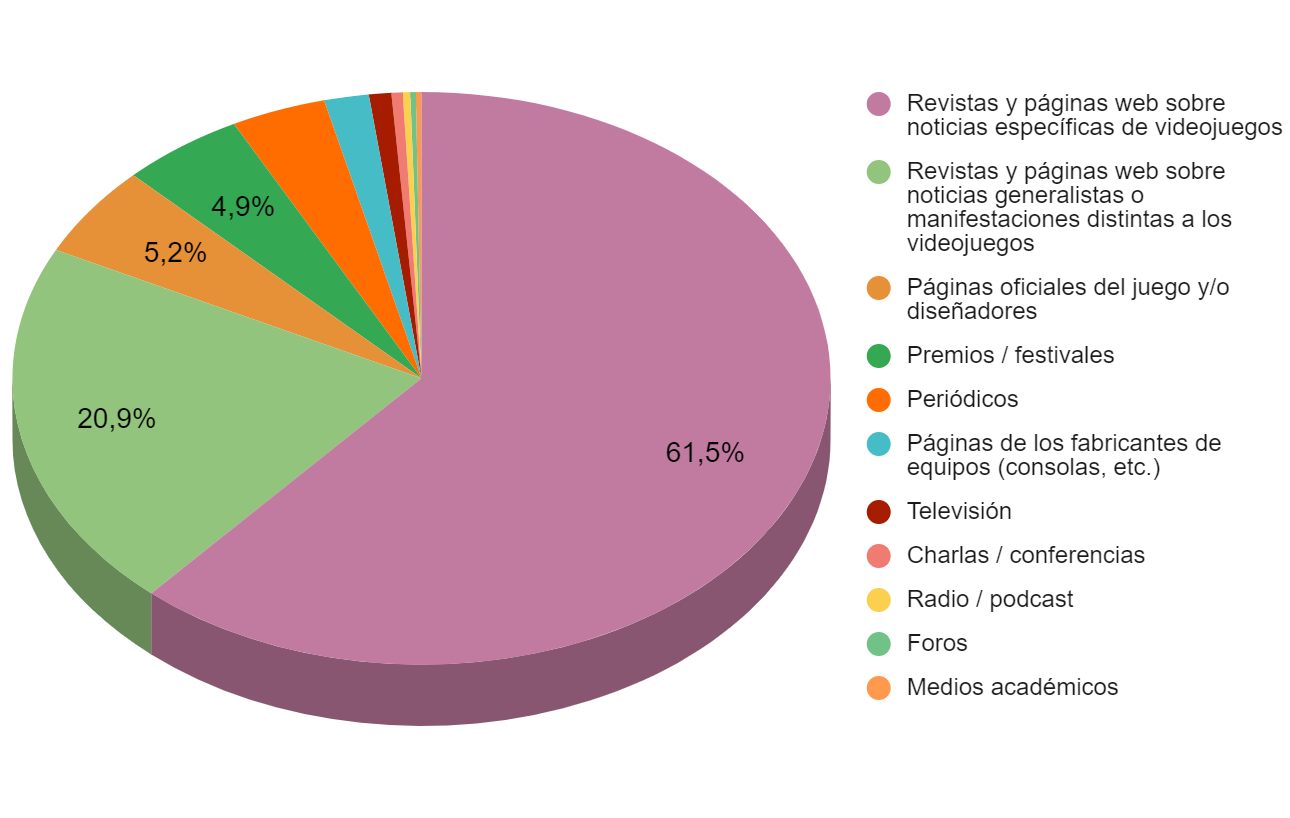
\includegraphics[width=\textwidth]{fig05.png}
 \source{Elaboración propia}
 \caption{Peso de las distintas categorías de medios utilizados como referencias en los artículos sobre videojuegos independientes}
 \label{fig05}
\end{minipage}
\end{figure}

Los editores de Wikipedia ponen en valor estos trabajos, reconociendo varios de ellos como "artículos buenos" o “artículos destacados”, los dos sistemas de reconocimiento existentes. En particular, cinco fueron nombrados como artículos buenos: \emph{Life is Strange} en inglés y portugués, \emph{Hellblade: Senua's Sacrifice} en ruso, \emph{Life Is Strange: Before the Storm} en inglés y vietnamita, \emph{Her Story} en inglés, ruso y sueco y \emph{Return of the Obra Dinn} en inglés, francés y ruso. Por su parte, \textit{Gone Home} fue nombrado como artículo destacado en sueco y \emph{A Short Hike} en francés.

Como veremos en el siguiente apartado, a pesar de este reconocimiento, la calidad de los mismos podría mejorar incluyendo fuentes más diversas y que entiendan el potencial educativo y artístico de los videojuegos independientes.



\section{Discusión y conclusiones}

Para dar respuesta a la primera pregunta de investigación partimos de 36 juegos independientes identificando los 28 que tenían información en Wikipedia en inglés. Esta labor curatorial puede, en sí misma, resultar de utilidad a los docentes, facilitándoles un pequeño repositorio al que acudir si buscan juegos comerciales para llevar al aula. Se trata, por lo tanto, de un trabajo en la línea de los realizados por \textcite{becker2017choosing} sobre la identificación de juegos comerciales con posibilidades educativas o \textcite{rojas-garcia_alisis_2022} al identificar experiencias en el contexto de educación secundaria.

Fue reconfortante comprobar la capacidad de Wikipedia para generar información sobre videojuegos independientes. En particular, el artículo de \emph{Life is Strange} es el que contiene más información y un mayor número de referencias. Era previsible que juegos como éste, que se mueven en la frontera entre lo independiente y lo mainstream, tuvieran artículos más grandes. No obstante, se trata de un juego que, a pesar del éxito de ventas, tiene un marcado carácter independiente si atendemos al tratamiento que hace de la memoria, el tiempo y las artes. Distintos autores han subrayado desde el ámbito académico su profundidad \cite{de_miranda_life_2018} así como las posibilidades educativas que ofrece en distintas asignaturas \cite{cantano2019educacion}. El juego, además, cuenta con artículos en Wikipedia para todos los episodios de la saga, así como para varios de sus personajes.

Como se explicaba en resultados, el tamaño de los artículos correlaciona de manera muy débil con su fecha de creación. Un ejemplo de esto sería \emph{Dreams}, que a pesar de ser galardonado en 2020 ocupa la sexta posición si atendemos a su extensión. Esto podría indicar que cuando un juego es particularmente creativo, como ocurre según \textcite{heaven_how_2019} con este título, puede obtener cierta repercusión mediática y atraer la atención de docentes y wikipedistas.

De hecho, fue una sorpresa comprobar que juegos tan disruptivos como \emph{Papers, please} o \emph{Her Story}, que poseen según distintos autors grandes posibilidades educativas \cite{cabellos_pro-social_2022} ocuparan posiciones tan altas. Por ejemplo, en \emph{Papers, please} ocupamos el rol de un oficial de aduanas en una ficticia república soviética y decidiremos, a partir de las instrucciones que recibimos cada día, qué personas pueden pasar y a quienes denegamos la entrada. Creemos que lo especial de las temáticas y mecánicas de estos juegos sirve como ejemplo para entender la creatividad del medio y las posibilidades que pueden ofrecer a los docentes en la línea apuntada por \textcite{hanghoj2020computerspil}.

Por su parte, \emph{Her Story} (ver \Cref{fig06}), desarrollado de forma autónoma por el británico Sam Barlow, simula el escritorio de un antiguo ordenador en una estación de policía en el que encontramos una carpeta con varios vídeos. Sin ninguna instrucción, el jugador ha de visualizarlos y reconstruir la historia de dos hermanas.

\begin{figure}[htbp]
\centering
\begin{minipage}{.85\textwidth}
 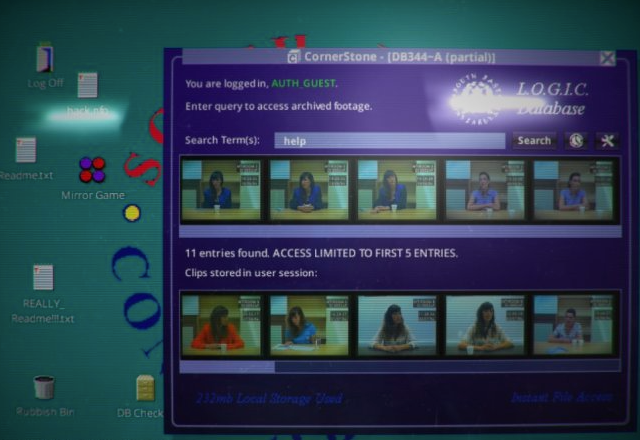
\includegraphics[width=\textwidth]{fig06.png}
 \caption{Captura de pantalla de Her Story}
 \label{fig06}
 \source{Sam Barlow}
\end{minipage}
\end{figure}

Al dar respuesta a la segunda pregunta de investigación comprobamos que los artículos, en particular los más grandes, poseen un elevado número de citas. A priori sería indicador de su calidad y de hecho la propia Wikipedia reconoce siete de ellos como artículos buenos o destacados (los reconocimientos más importantes otorgados por la comunidad de editores a los artículos). No obstante, sería interesante que esta interpretación de calidad dependiera de criterios diversos y, sobre todo, que entendiera la riqueza del medio, así como su dimensión artística y educativa. En este sentido podría valorarse la inclusión de citas del ámbito académico frente al uso exclusivo de referencias populares. En los últimos años, Wikipedia ha realizado esfuerzos significativos para mejorar su reputación como fuente fiable de información \cite{sahut_wikipedia:_2017} guiándose por el hecho de que la mayoría de usuarios la consideren una fuente valida. Aunque \textcite{colavizza_covid-19_2020} ha sido uno de los defensores de la calidad de la Wikipedia afirmando que sus artículos contienen un gran número de referencias pertenecientes a publicaciones científicas respetables, en el caso de nuestros juegos, muchas veces, éstas pertenecen a revistas y páginas web de videojuegos, en ocasiones de dudosa calidad.

De hecho, al responder a la tercera pregunta de investigación y analizar las 1358 referencias de las que se nutren los artículos, comprobamos que la mayoría pertenecían a revistas y páginas web cuyo foco estaba, paradójicamente, en juegos súper ventas (61.5\%). La investigación ha demostrado que este tipo de publicaciones (revistas como \emph{Hardcore Gamer} que ocupa la undécima posición con 20 referencias) consolidan estereotipos identitarios al dar visibilidad casi exclusiva a determinados géneros (guerra, lucha, juegos deportivos, etc.) frente a otros, asociándolos a lo que se considera ser jugador \cite{shaw_you_2012, vilasis-pamos_how_2021}. Afortunadamente, encontramos otros medios que comienzan a tratar los videojuegos con una nueva sensibilidad \cite{suter_narrative_nodate}. Entre estos podemos citar páginas web como \emph{Polygon} (segundo lugar y 90 referencias), la evolución que en los últimos años ha sufrido \emph{Eurogamer} (quinto lugar y 61 referencias) y, en particular, \emph{Gamasutra} (séptimo lugar y 39 referencias), dirigida a los diseñadores de juegos.

Aunque la inclusión de referencias de estos medios nos parece positiva, a la hora de dar respuesta a la última pregunta de investigación comprobamos que las revistas de videojuegos (incluidas muchas de baja calidad) y los medios generalistas son las categorías en las que se encuadran la mayoría de referencias, siendo alarmante la ausencia de contenido científico. Esto implica la ausencia de libros (no exclusivamente académicos), actas de congresos y revistas académicas revisadas por pares. En esta línea, \textcite{kousha_are_2017} ha apuntado que la utilización de artículos científicos en el contenido de Wikipedia sigue siendo escasa. Llama la atención la ausencia de contenido vinculado a las ciencias de la educación, los game studies y el aprendizaje basado en juegos.

Somos conscientes de que nos hallamos ante juegos que, más allá de su dimensión estética y emocional y de las posibilidades educativas que ofrecen, son productos de entretenimiento con una finalidad lúdica. Podría pensarse, por lo tanto, que la ausencia de referencias académicas, en general, y de las ciencias de educación, los game studies y el aprendizaje basado en juegos, en particular, son incluso lógicas. Sin embargo, desde nuestra óptica, estas ausencias se deben a sesgos y estereotipos que impiden ver los juegos como manifestaciones artísticas con posibilidades educativas. Si los comparamos con otros medios vemos que, desde hace años, existe un corpus científico que reconoce el valor cultural e histórico del cine como medio artístico, así como sus posibilidades educativas \cite{pegrum_contemporary_2005}. Por otro lado, si nos centramos en Wikipedia, un simple acceso al artículo “Cinematografía” en inglés, permite comprobar que se nutre de gran cantidad de referencias pertenecientes al ámbito académico, apareciendo libros, revistas académicas y actas de congresos. En la misma línea, un acceso al artículo “Educación mediática”, muestra múltiples menciones al cine y ninguna a los videojuegos. Creemos que todo esto es representativo de lo infravalorados que continúan estando los juegos como productos artísticos con posibilidades educativas, tanto en Wikipedia como en los medios de comunicación.

En lo que respecta a Wikipedia, podría ser interesante que sus editores y los grupos especializados en juegos (como el “WikiProject Video Games” que trabaja en más de 37 idiomas), consideraran la utilización de estas fuentes y que se acercaran a los juegos entendiéndolos como productos análogos al cine o la literatura.

Por otro lado, es necesario entender que los medios de comunicación continúan centrándose en cuestiones como los altos niveles de violencia o potenciales adicciones, representando el medio únicamente con fenómenos como los \emph{esports} o los últimos lanzamientos comerciales triple A (\emph{Call of Duty, FIFA}, etc.). Incluso, en ocasiones, se establecen relaciones directas entre atentados perpetrados por adolescentes y su condición de jugadores, como ocurrió, en su momento, con la matanza de Columbine o, más recientemente, con el asesinato de 21 personas en una escuela de Texas \cite{gallego2022}.

Siguiendo a \textcite{egenfeldt2021understanding}, consideramos que este sensacionalismo se basa en interpretaciones reduccionistas del corpus teórico denominado perspectiva del medio activo (acercamientos psicologistas que consideran los juegos como un medio con capacidad para generar adicciones y provocar violencia por sí mismo) frente a la perspectiva del usuario activo (enfoques que ponen en valor la agencia del usuario y su capacidad para hacer un uso responsable y positivo del medio).

Este trabajo presenta varias limitaciones. La primera de ellas está vinculada al tamaño muestral dado que podrían incluirse más certámenes, más juegos y, por extensión, más artículos de Wikipedia. No obstante, la elección de 2014 como fecha de corte no es aleatoria y se basa en la creación del certamen Games for Change, así como en la consolidación de los términos juegos independientes e indie games en la cultura popular durante esos años. Otra limitación (que llevó también a acotar el tamaño muestral) es el trabajo manual de categorización realizado por los autores y que, como tal, puede estar expuesto a sesgos de distinto tipo. Por ello, una prometedora línea de trabajo es la introducción de técnicas de machine learning, inteligencia artificial y programación como complemento de la labor de los investigadores. Actualmente nos encontramos explorando esta posibilidad, realizando los primeros scripts que permitan automatizar procesos a la hora de obtener datos de Wikipedia.

Esperamos que este trabajo contribuya a poner en valor los tímidos esfuerzos hechos hasta la fecha para reivindicar los juegos independientes y sus posibilidades educativas. En particular su potencial para ser utilizados desde una perspectiva sociocultural y, sobre todo, con el foco en el engagement emocional y afectivo que pueden generar \cite{plass_foundations_2015}. Los trabajos en este sentido son escasos. Resultan particularmente interesantes las experiencias de \textcite{hanghoj2020computerspil} con \emph{Limbo} y, en el contexto español, las propuestas de \textcite{oceja_playing_2021} con \emph{Braid y Gris} o las de \textcite{hidalgo2022} con \emph{RiME}. Estos trabajos se enmarcan dentro del proyecto educativo Playing Emotions, que la Fundación Botín tiene implementado en distintos lugares de España e Iberoamérica para promover competencias afectivo-emocionales (autoestima, empatía, identificación emocional, etc.) desde distintas asignaturas a través de los juegos independientes.

A día de hoy, nadie cuestiona las posibilidades educativas del cómic, el cine o la literatura y, sin embargo, los docentes no escogen productos comerciales y de consumo rápido. En su lugar, entienden la complejidad de estos medios, son conscientes de su valor creativo y de su capacidad para conmovernos, y por ello realizan una labor curatorial que les permite trabajar con piezas de gran potencial educativo. Aunque esto mismo debería ocurrir con los videojuegos, la visión de los medios de comunicación dificulta esta labor. Como consecuencia, una gran cantidad de juegos cargados de creatividad, talento y sentido artístico, son desconocidos por los docentes. Incluso analizando la literatura científica es difícil localizar proyectos de corte educativo que aboguen por el uso de estos juegos desde una perspectiva sociocultural y buscando la implicación afectiva y emocional de los jugadores.

Esta visión sesgada de los videojuegos supone un cóctel explosivo que amenaza con perpetuar su estigmatización. Por ello es importante la aparición en el panorama mediático de voces que se acerquen a este producto de una forma madura y sin sensacionalismos.

Si la comunidad científica, los medios de comunicación y Wikipedia reinterpretan el papel de los videojuegos en nuestra sociedad y reconocen su valor como artefactos culturales y artísticos con posibilidades educativas, el escenario podría ser muy diferente. Tal vez entonces se den las condiciones adecuadas para que los educadores exploren la diversidad y riqueza de los videojuegos creando en sus aulas experiencias dialógicas y transformadoras.












 














\printbibliography\label{sec-bib}
% if the text is not in Portuguese, it might be necessary to use the code below instead to print the correct ABNT abbreviations [s.n.], [s.l.]
%\begin{portuguese}
%\printbibliography[title={Bibliography}]
%\end{portuguese}


%full list: conceptualization,datacuration,formalanalysis,funding,investigation,methodology,projadm,resources,software,supervision,validation,visualization,writing,review
\begin{contributors}[sec-contributors]
\authorcontribution{Jorge Oceja}[conceptualization,datacuration,writing]
\authorcontribution{Ángel Obregón Sierra}[conceptualization,methodology,software]
\end{contributors}


\end{document}

